\pdfminorversion 4
%% otherwise pdftk does not run properly...
\documentclass[10pt]{beamer}\usepackage[]{graphicx}\usepackage[]{color}
%% maxwidth is the original width if it is less than linewidth
%% otherwise use linewidth (to make sure the graphics do not exceed the margin)
\makeatletter
\def\maxwidth{ %
  \ifdim\Gin@nat@width>\linewidth
    \linewidth
  \else
    \Gin@nat@width
  \fi
}
\makeatother

\definecolor{fgcolor}{rgb}{0.345, 0.345, 0.345}
\newcommand{\hlnum}[1]{\textcolor[rgb]{0.686,0.059,0.569}{#1}}%
\newcommand{\hlstr}[1]{\textcolor[rgb]{0.192,0.494,0.8}{#1}}%
\newcommand{\hlcom}[1]{\textcolor[rgb]{0.678,0.584,0.686}{\textit{#1}}}%
\newcommand{\hlopt}[1]{\textcolor[rgb]{0,0,0}{#1}}%
\newcommand{\hlstd}[1]{\textcolor[rgb]{0.345,0.345,0.345}{#1}}%
\newcommand{\hlkwa}[1]{\textcolor[rgb]{0.161,0.373,0.58}{\textbf{#1}}}%
\newcommand{\hlkwb}[1]{\textcolor[rgb]{0.69,0.353,0.396}{#1}}%
\newcommand{\hlkwc}[1]{\textcolor[rgb]{0.333,0.667,0.333}{#1}}%
\newcommand{\hlkwd}[1]{\textcolor[rgb]{0.737,0.353,0.396}{\textbf{#1}}}%

\usepackage{framed}
\makeatletter
\newenvironment{kframe}{%
 \def\at@end@of@kframe{}%
 \ifinner\ifhmode%
  \def\at@end@of@kframe{\end{minipage}}%
  \begin{minipage}{\columnwidth}%
 \fi\fi%
 \def\FrameCommand##1{\hskip\@totalleftmargin \hskip-\fboxsep
 \colorbox{shadecolor}{##1}\hskip-\fboxsep
     % There is no \\@totalrightmargin, so:
     \hskip-\linewidth \hskip-\@totalleftmargin \hskip\columnwidth}%
 \MakeFramed {\advance\hsize-\width
   \@totalleftmargin\z@ \linewidth\hsize
   \@setminipage}}%
 {\par\unskip\endMakeFramed%
 \at@end@of@kframe}
\makeatother

\definecolor{shadecolor}{rgb}{.97, .97, .97}
\definecolor{messagecolor}{rgb}{0, 0, 0}
\definecolor{warningcolor}{rgb}{1, 0, 1}
\definecolor{errorcolor}{rgb}{1, 0, 0}
\newenvironment{knitrout}{}{} % an empty environment to be redefined in TeX

\usepackage{alltt}
\usetheme{PaloAlto}
\usecolortheme{beaver}
\usepackage[english]{babel}
\usepackage[utf8]{inputenc}
\usepackage[T1]{fontenc}
\usepackage{graphicx}  
\usepackage[scaled=1]{helvet} 
\usepackage{fancyvrb}
\usepackage{fixltx2e}
\usepackage{amsmath}
\graphicspath{{pics/}}                  % path to graphics
\beamertemplatenavigationsymbolsempty
\setbeamercovered{transparent}% Allow for shaded (transparent) covered items



%% Custumizations of theme
% Bold font in titles
\setbeamerfont{frametitle}{series=\bfseries} 
\setbeamerfont{block title}{series=\bfseries}

\setbeamercolor{section in sidebar}{fg=black}
\setbeamercolor{title in sidebar}{fg=black}

\setbeamertemplate{itemize items}[default]
\setbeamercolor*{item}{fg=darkred} % all frames will have red bullets

\renewcommand{\footnotesize}{\scriptsize}


% customize color code chunk (Scode = inline)
\definecolor{Sinput}{rgb}{0.75,0.19,0.19}
\definecolor{Soutput}{rgb}{0,0,0}
\definecolor{Scode}{rgb}{0.75,0.19,0.19}


\title{PERMANOVA}
\author{Eduard Szöcs}
\institute{Institute for Environmental Sciences - University Koblenz-Landau}
\date{\today}
\logo{
\includegraphics[width = 1.5cm]{logo.pdf}}
\IfFileExists{upquote.sty}{\usepackage{upquote}}{}
\begin{document}
% default size for the sweaved graphics
%\setkeys{Gin}{width=1\textwidth}
% default font size and color for R code
\DefineVerbatimEnvironment{Sinput}{Verbatim}{formatcom = {\color{Sinput}},fontsize=\scriptsize}
\DefineVerbatimEnvironment{Soutput}{Verbatim}{formatcom = {\color{Soutput}},fontsize=\footnotesize}
\DefineVerbatimEnvironment{Scode}{Verbatim}{formatcom = {\color{Scode}},fontsize=\small}

%%% Setup structure and load data and pacakges





%%% Begin slides
%% Title Page
\begin{frame} 
  \titlepage
\end{frame}

\section{Introduction}
\begin{frame}
  \frametitle{Introduction}
  \begin{itemize}
    \item Assumptions of MANOVA:
    \begin{itemize}
      \item Independence of the sample units 
      \item Multivariate normality 
      \item Homogeneity of variance–covariance matrices 
    \end{itemize} 
    \item Euclidean distance useful? \pause
    \item Generally \textbf{not} met for ecological data sets!
    \item Need a robust method to handle complex data sets.
  \end{itemize}
\end{frame}

\begin{frame}
  \frametitle{Permutational Multivariate Analysis of Variance Using Distance Matrices}
  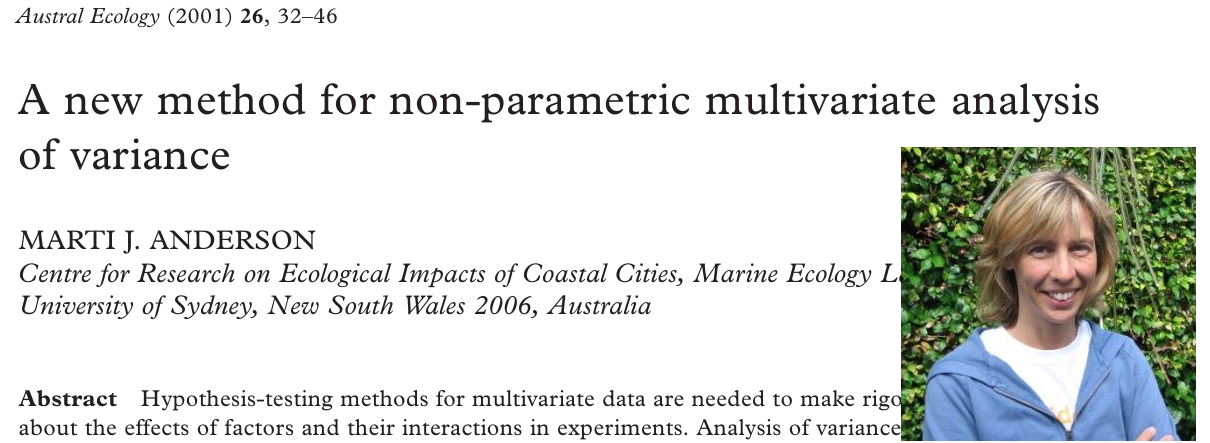
\includegraphics[width = \textwidth]{both.jpg}
  \pause
  \begin{itemize}
    \item Very influential paper in community ecology
    \begin{itemize}
      \item Google Scholar: >4500 citations
    \end{itemize}
    \pause
    \item Non-parametric approach combined with ecological distance measures!
  \end{itemize}
\end{frame}

\subsection{Data}
\begin{frame}
  \frametitle{Data set used in this lecture}
  Macroinvertebrate data from the River Werra\footnotemark \footnotetext{Bäthe, Jürgen, and Eckhard Coring. Biological Effects of Anthropogenic Salt-load on the Aquatic Fauna: A Synthesis of 17 Years of Biological Survey on the Rivers Werra and Weser. Limnologica - Ecology and Management of Inland Waters 41(2): 125-133.}

  \textcolor{darkred}{Aim :} Effect of anthropogenic salinisation on macroinvertebrate communities 

  \begin{columns}
  \begin{column}{5cm}
    \begin{itemize}
      \item upstream - downstream design
      \item salt brine discharge around Vacha
      \item Do the communities differ between up- and downstream?
      \item Not the original data (proprietary).
    \end{itemize}
  \end{column}
  \begin{column}{5cm}
      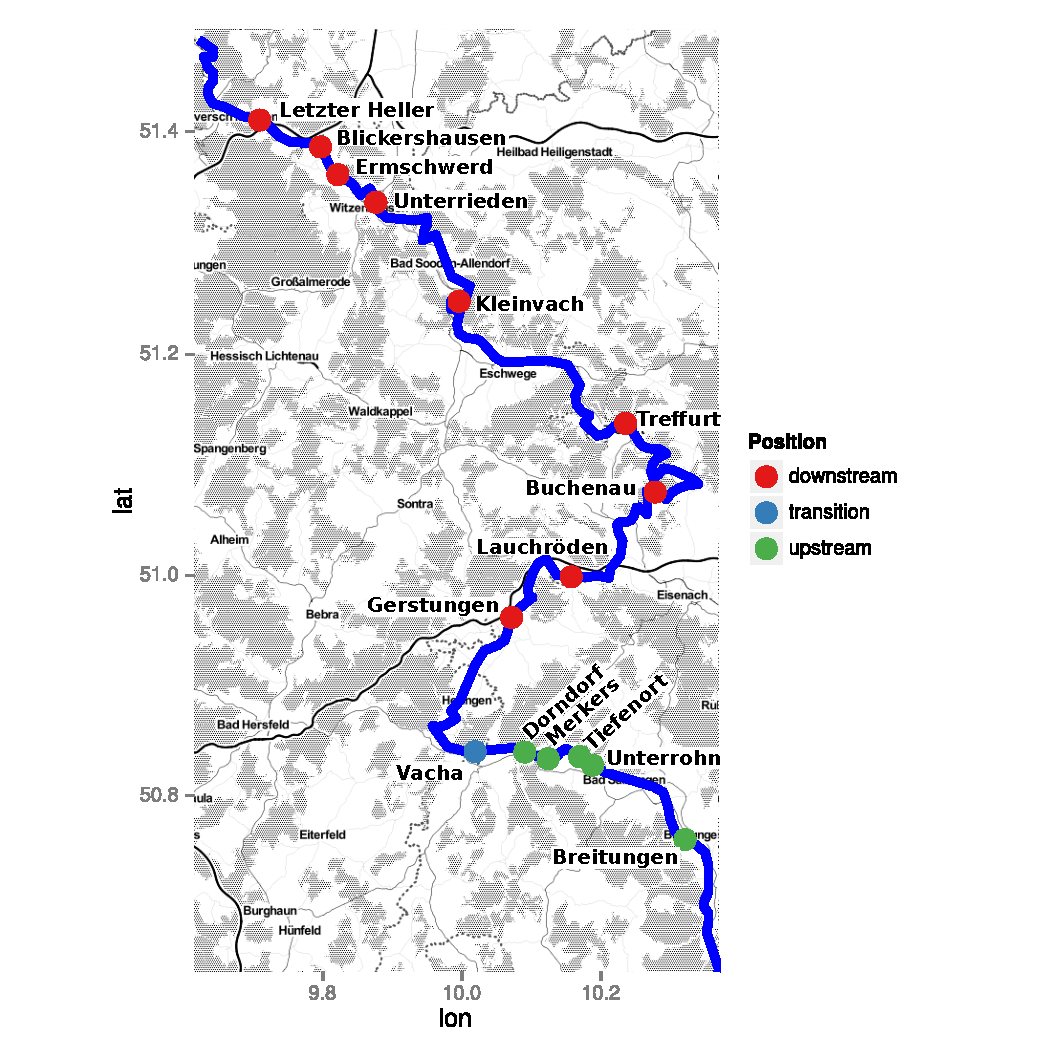
\includegraphics[height=0.7\textheight]{pics/map.pdf}
      \footnotemark
\end{column}
\end{columns}
\end{frame}

\begin{frame}[fragile]
\frametitle{First impression of the data}
\begin{itemize}
  \item NMDS Bray-Curtis-Distance and x\textsuperscript{0.25} transformation. 
\end{itemize}
  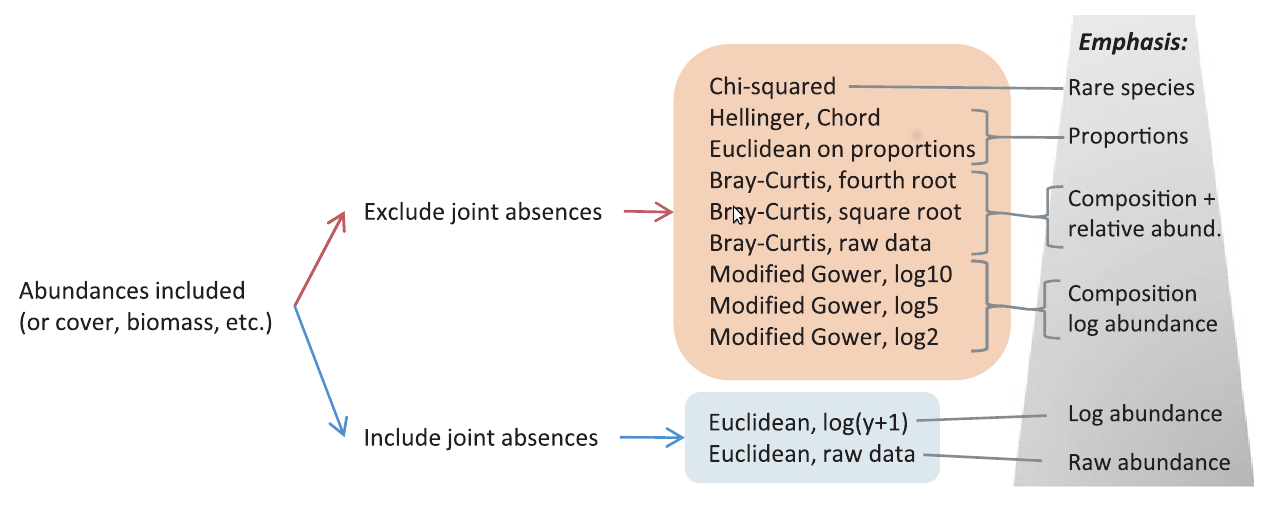
\includegraphics[width=.9\linewidth]{dt.png}
  \footnote{Anderson MJ, Crist TO, Chase JM, Vellend M, Inouye BD, Freestone AL, et al. Navigating the multiple meanings of beta diversity: a roadmap for the practicing ecologist. Ecology Letters. 2011;14(1):19–28. }
\end{frame}

\begin{frame}[fragile]
\frametitle{First impression of the data - NMDS}
\begin{itemize}
  \item NMDS Bray-Curtis-Distance and x\textsuperscript{0.25} transformation. 
\end{itemize}

 \begin{columns}
  \begin{column}{5cm}
    \begin{itemize}
    \item upstream and downstream sites clearly separate in NMDS.
    \item Spread looks similar.
    \item Indication of a difference between upstream and downstream.
    \end{itemize}
  \end{column}
  \begin{column}{5cm}
\begin{knitrout}\footnotesize
\definecolor{shadecolor}{rgb}{0.969, 0.969, 0.969}\color{fgcolor}

{\centering 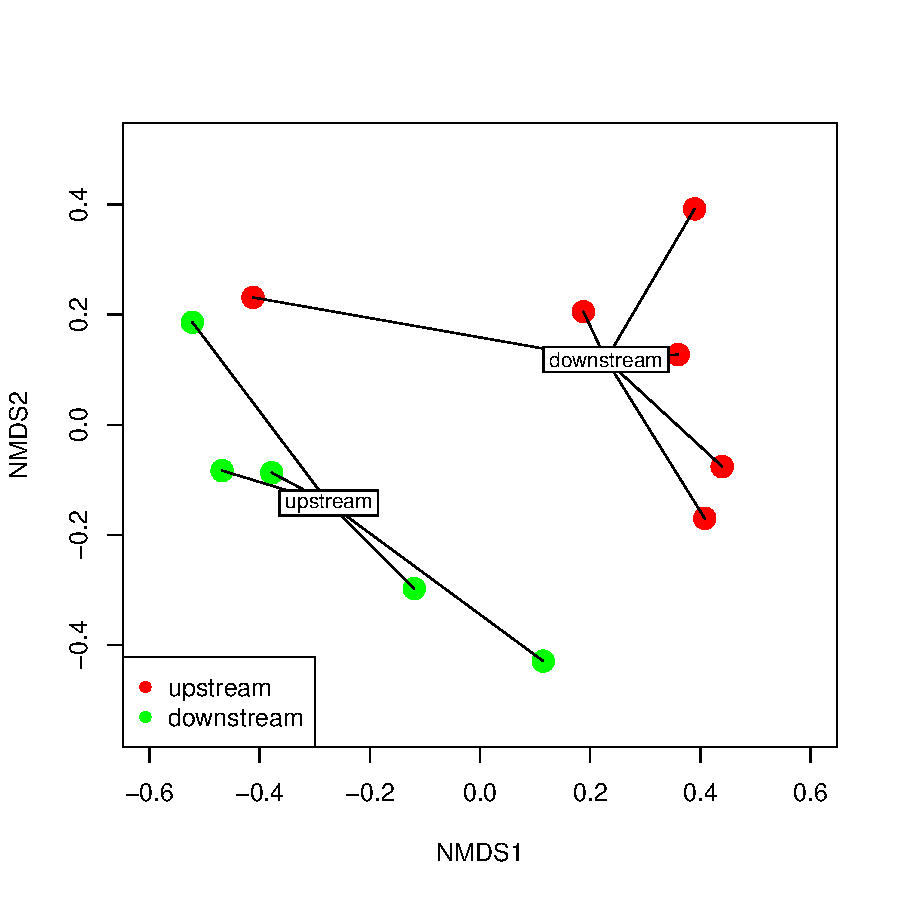
\includegraphics[width=5cm,height=5cm]{figs/nmds2_plot-1} 

}



\end{knitrout}
    \end{column}
  \end{columns}
\end{frame}

\section{Maths}
\begin{frame}[fragile]
  \frametitle{Recap: ANOVA}
  \textcolor{darkred}{Question :} How is univariate ANOVA calculated?
  \begin{block}{From univariate...}
  \begin{columns}
  \begin{column}{5cm}
\begin{knitrout}\footnotesize
\definecolor{shadecolor}{rgb}{0.969, 0.969, 0.969}\color{fgcolor}

{\centering 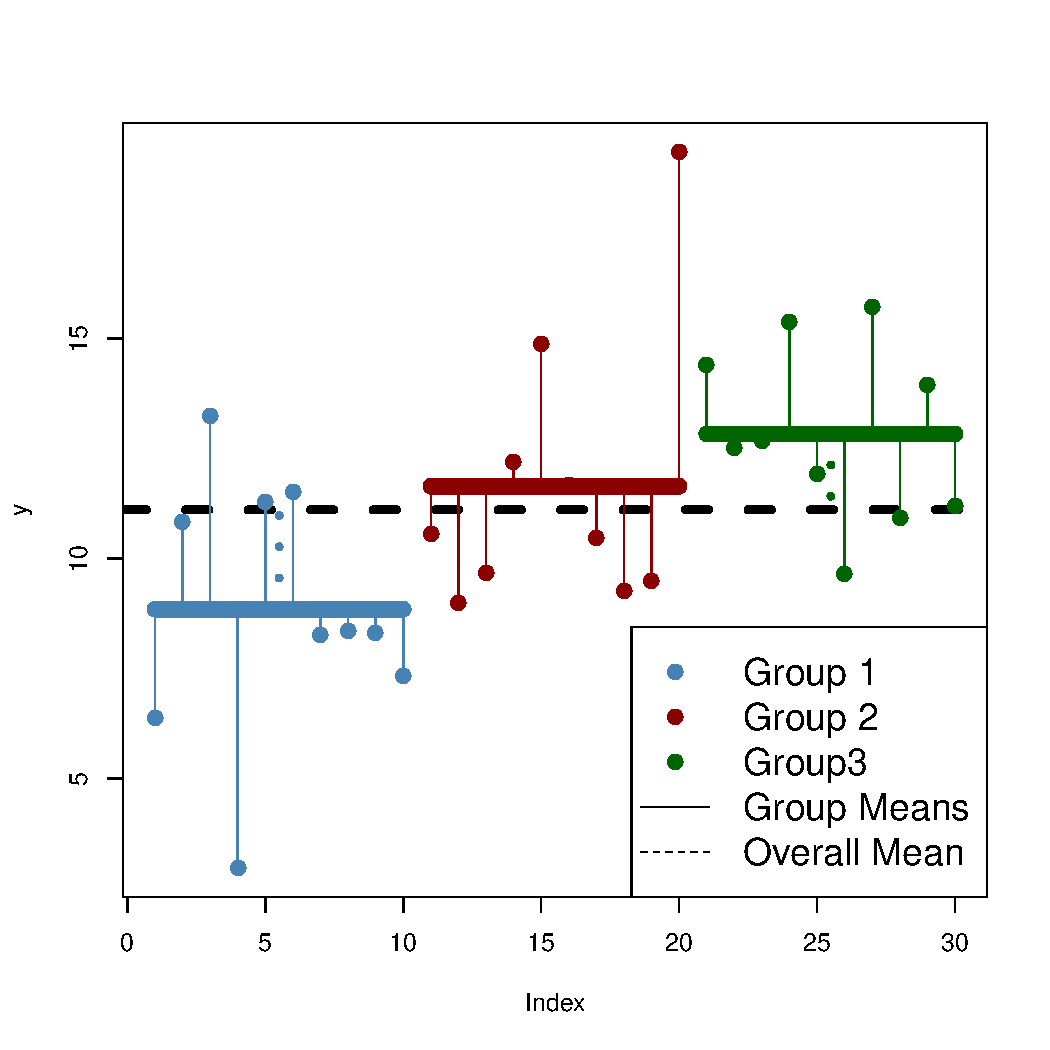
\includegraphics[width=\maxwidth]{figs/permanova1-1} 

}



\end{knitrout}
  \end{column}
  \pause
  \begin{column}{5cm}
  $F-ratio = \frac{SS_{group}}{SS_{residual}} \cdot \frac{df_{residual}}{df_{group}}$\\[0.5em]
  \small $SS_{total} = SS_{residual} + SS_{group}$
  \visible<3->{
\begin{knitrout}\footnotesize
\definecolor{shadecolor}{rgb}{0.969, 0.969, 0.969}\color{fgcolor}

{\centering 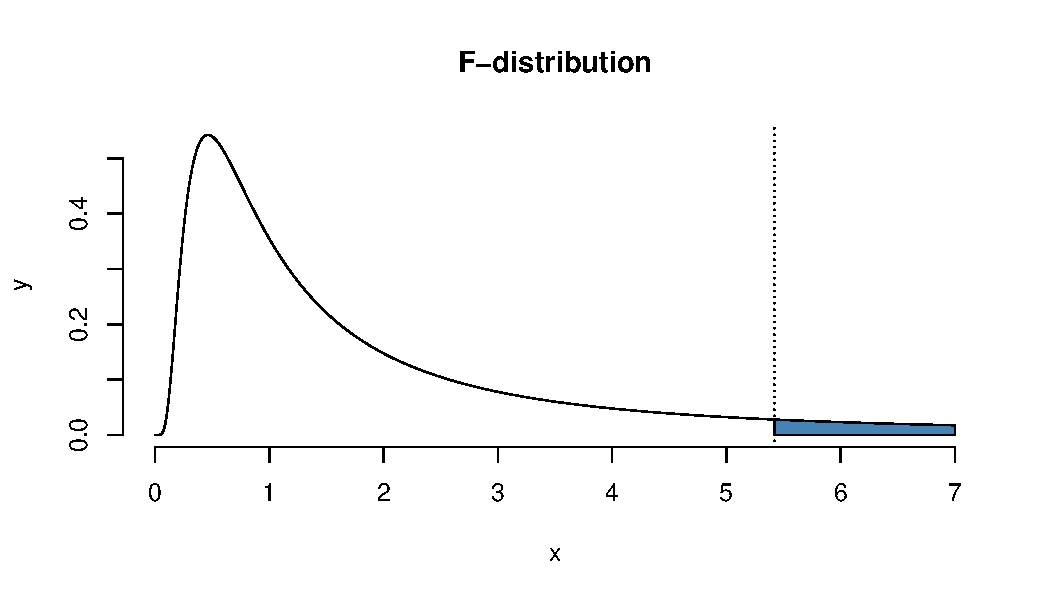
\includegraphics[width=\maxwidth]{figs/F-distr-1} 

}



\end{knitrout}
  }
  \end{column}
  \end{columns}
  \end{block}
\end{frame}

\begin{frame}[fragile]
  \frametitle{Distance-based MANOVA}
Distance-based MANOVA is analogous!
  \begin{block}{... to multivariate ANOVA}
  \begin{columns}
  \begin{column}{5cm}
\begin{knitrout}\footnotesize
\definecolor{shadecolor}{rgb}{0.969, 0.969, 0.969}\color{fgcolor}

{\centering 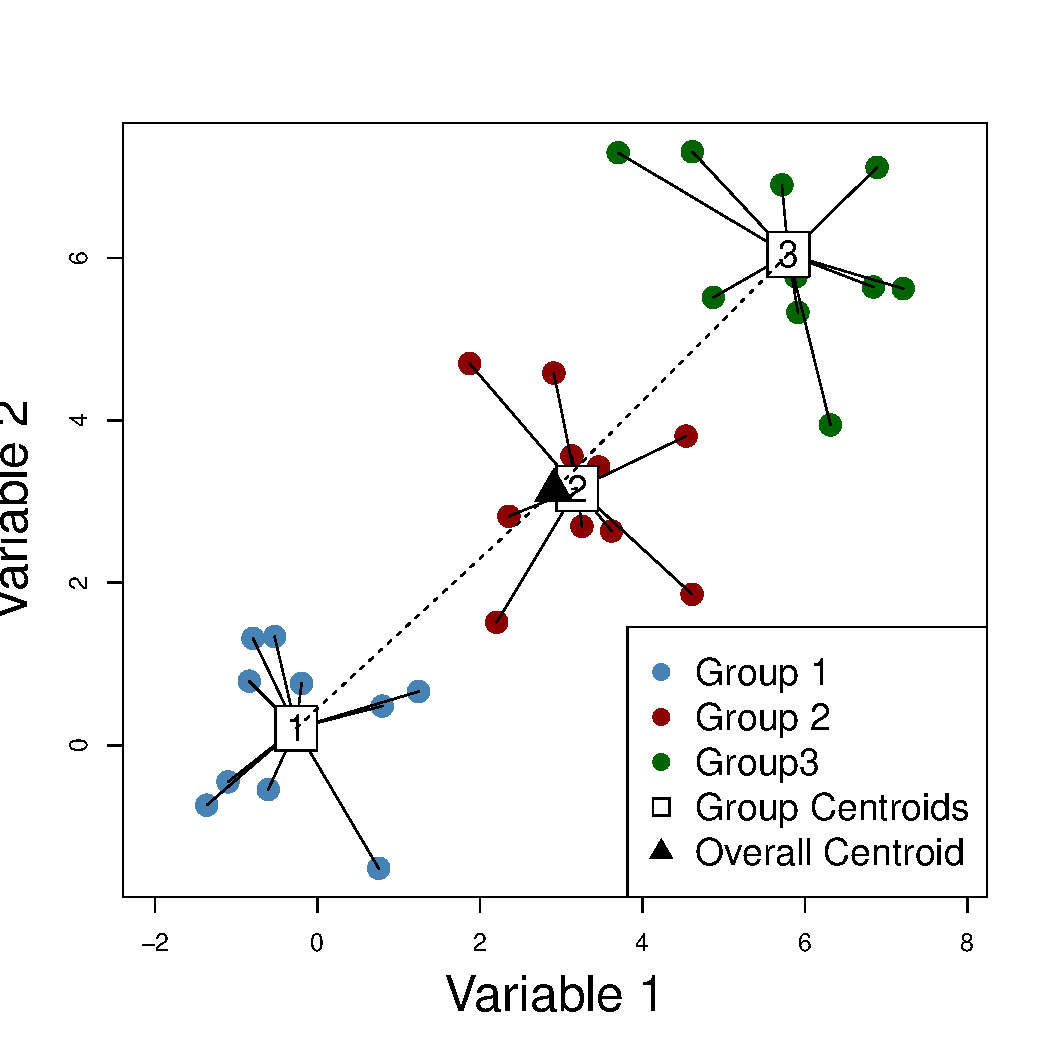
\includegraphics[width=\maxwidth]{figs/permanova2-1} 

}



\end{knitrout}
      \end{column}
      \begin{column}{5cm}
      \begin{itemize}
      \item Partitioning into variance components:\\
            $SS_{total} = SS_{group} + SS_{residual}$
      \item \textbf{centroids}
      \item p-value by \textbf{permutations}
      \end{itemize}
      \end{column}
  \end{columns}
  \end{block}
\end{frame}

\begin{frame}[fragile]
  \frametitle{Variance Partitioning}
  \begin{itemize}
  \item We can use any \textbf{Distance Matrix} to partition the variance.
  \pause
  \item \textcolor{blue}{Sum of squared distances from individual points to their centroid} is equal to the \textcolor{red}{sum of squared interpoint distances divided by the number of points}.
   
  \item $\textcolor{blue}{\sum d_{i-centroid}^2} = \textcolor{red}{\frac{1}{N}\sum d_{i-j}^2}$
  \end{itemize}
  \begin{centering}
  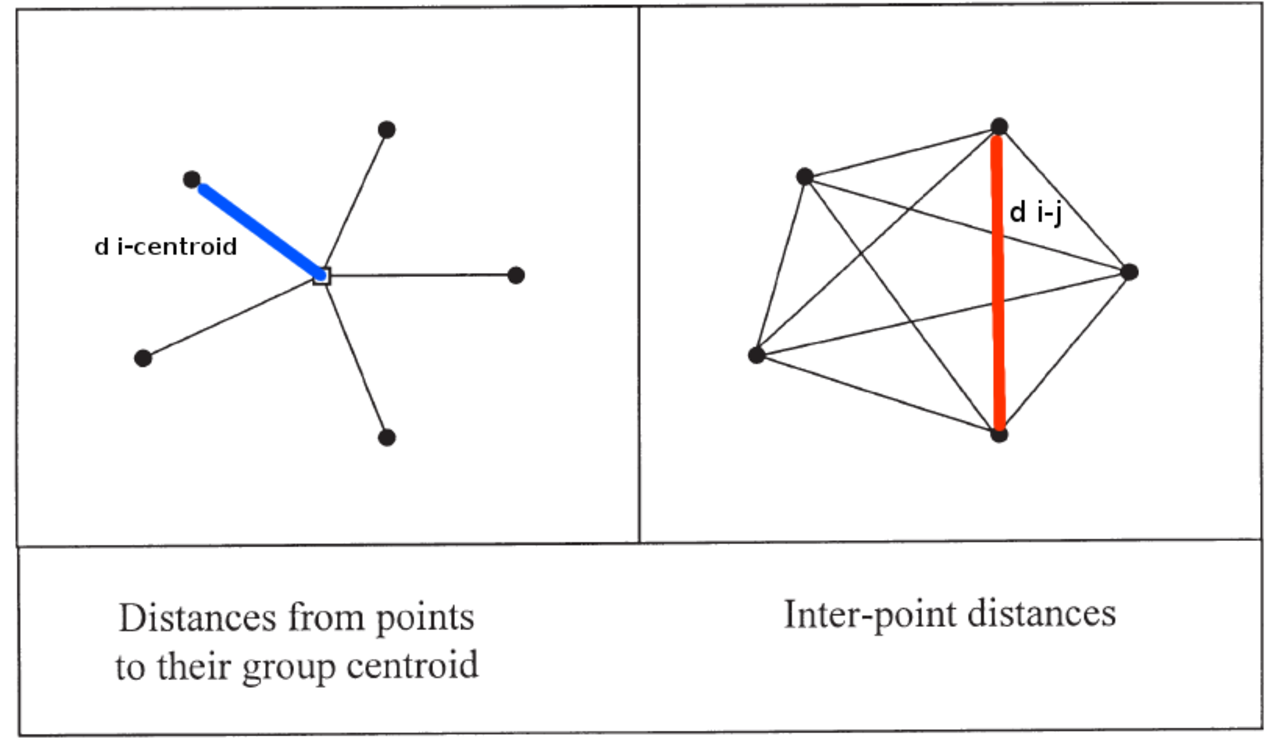
\includegraphics[height=0.5\textheight]{pics/Anderson_2001_ip.pdf}
  \end{centering}
\end{frame}


\begin{frame}[fragile]
  \frametitle{Variance Partitioning}
  Like in univariate ANOVA variance can be partitioned:
  \begin{columns}
  \begin{column}{5cm}
    \includegraphics<1->[height=0.4\textheight]{pics/Anderson_2001_SST.pdf}\\
    \visible<2->{
    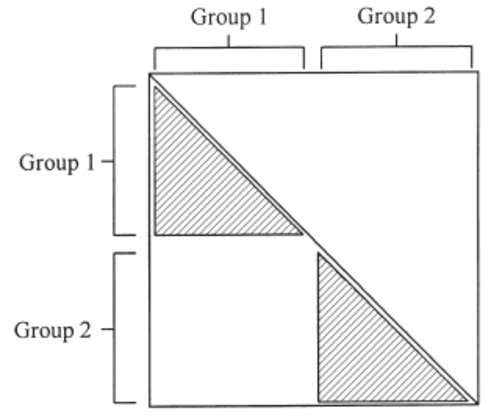
\includegraphics[height=0.4\textheight]{pics/Anderson_2001_SSG.pdf}
    }
  \end{column}
  \begin{column}{5cm}
  $SS_{total} = \frac{1}{N} \sum\limits_{i=1}^{N-1} \sum\limits_{j=i+1}^{N} d_{ij}^2$ \\
  \tiny N = total number of observations \\[2em] \normalsize \pause
  $SS_{residual} = \frac{1}{n} \sum\limits_{i=1}^{N-1} \sum\limits_{j=i+1}^{N} d_{ij}^2 \epsilon_{ij}$\\
  \tiny n = number of observations per group \\ 
  $\epsilon_{ij} = 
  \begin{cases}
    1,& \text{if }  \text{if observations i and j are in the same group}\\
    0,& \text{otherwise}
  \end{cases}$ \\[2em] \normalsize \pause
  
  $SS_{group} = SS_{total} - SS_{residual}$ \\[2em] \pause
  $(Pseudo-) F = \frac{SS_{group}}{SS_{residual}} \frac{N-a}{a-1}$\\
  
  \tiny a = no. groups\\[1em]
  \footnotesize
  p-value is assessed via permutations.
  \end{column}
  \end{columns}
\end{frame}


\begin{frame}
\frametitle{p-values using permutations}
\begin{columns}
  \begin{column}{5cm}
    \begin{itemize}
    \item Cannot use Fisher's F-ratio
      \begin{itemize}
        \item normal distribution?
        \item euclidean distance?
      \end{itemize} \vspace{1.5em} 
      \pause
      \item Instead use \textbf{permutations}
      \begin{itemize}
        \item shuffle data randomly
        \item compute F-Ratio ($F_{perm}$)
        \item repeat many times
      \end{itemize}\vspace{1.5em}
      \item compare  \textcolor{blue}{F of randomized data} with \textcolor{red}{original F}.\\[1.5em]
      \item $p = \frac{\text{No. of }F_{perm}~\ge~F}{\text{No. of permutations + 1}}$
    \end{itemize}
  \end{column}
  \begin{column}{5cm}
  \visible<2->{
\begin{knitrout}\footnotesize
\definecolor{shadecolor}{rgb}{0.969, 0.969, 0.969}\color{fgcolor}

{\centering 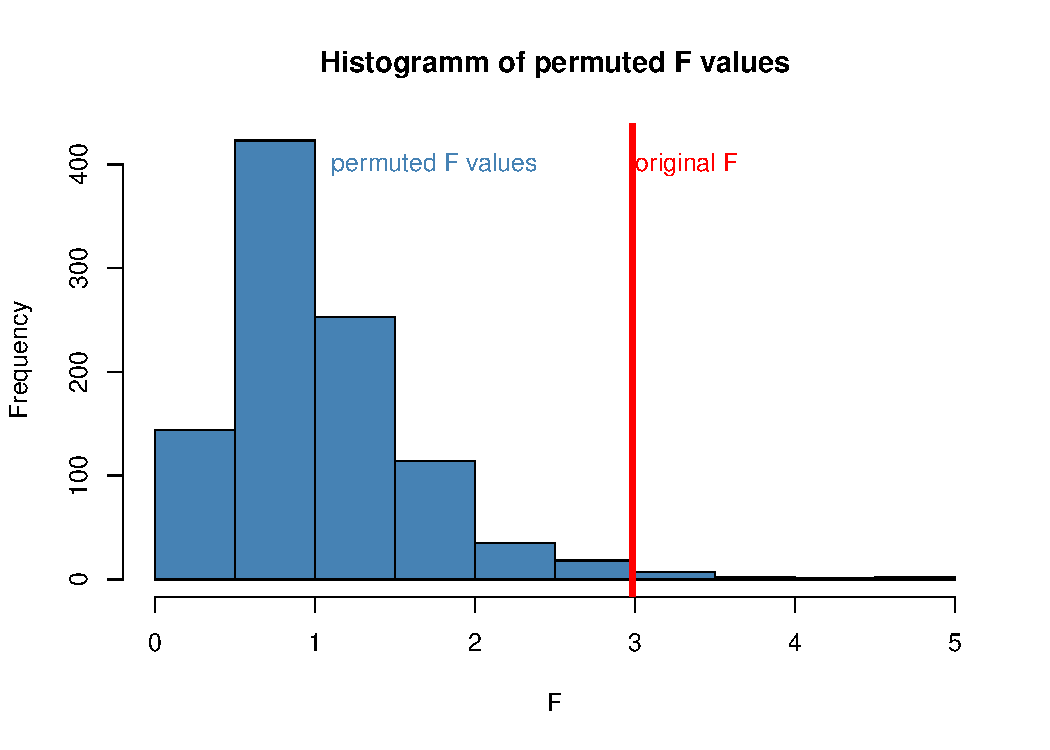
\includegraphics[width=\maxwidth]{figs/permplot-1} 

}



\end{knitrout}
}
  \end{column}
\end{columns}
\end{frame}

\section{Assumptions}
\begin{frame}[fragile]
  \frametitle{Assumptions of PERMANOVA}
\begin{columns}
  \begin{column}{5cm}
    \begin{itemize}
      \item equal \textbf{dispersions}
      \item Visual inspection
      \item Multivariate analogue to Levene's test available.\footnotemark
    \end{itemize}
    \pause
    \begin{itemize}
    \item Multivariate Dispersion
      \begin{itemize}
      \item $\beta$-diversity
      \item functional diversity
      \item see literature folder
      \end{itemize}
    \end{itemize}

  \end{column}
  \begin{column}{5cm}
\begin{knitrout}\footnotesize
\definecolor{shadecolor}{rgb}{0.969, 0.969, 0.969}\color{fgcolor}

{\centering 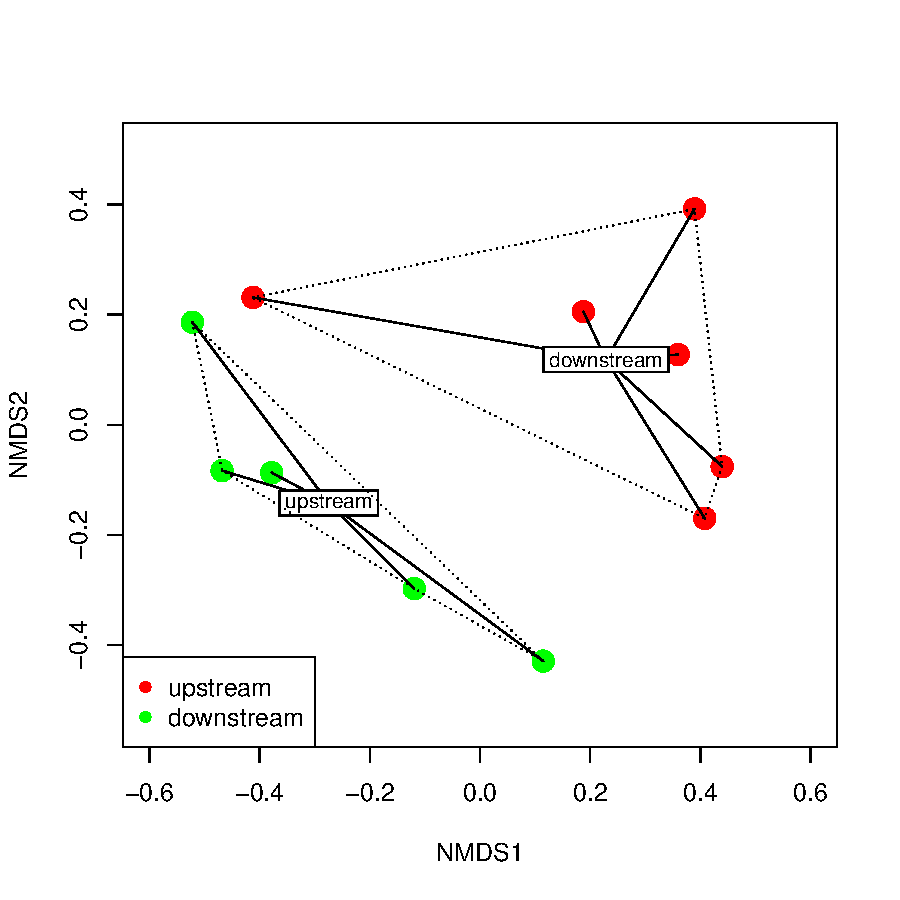
\includegraphics[width=5cm,height=5cm]{figs/nmds2_plot2-1} 

}



\end{knitrout}
    \end{column}
  \end{columns}
  \footnotetext{Anderson, M. J. 2006. Distance Based Tests for Homogeneity of Multivariate Dispersions. Biometrics 62 (1): 245-253.}
\end{frame}

% \section{SIMPER}
% \begin{frame}
% \frametitle{SIMPER - Which species are discriminating between the groups?}
% \begin{itemize}
%   \item Bray Curtis dissimilarity between two sites can be written as:
%   $$d_{ij} = \frac{\sum\limits_{k=1}^n |x_{jk} - x_{ik}|}{\sum\limits_{k=1}^n (x_{jk}+x_{ik})}$$
%   \pause
%   \item nominator is the sum of individual species (k) differences therefore the single contribution of species k is:
%   $$d_{ijk} = \frac{|x_{jk} - x_{ik}|}{\sum\limits_{k=1}^n (x_{jk}+x_{ik})}$$
%   \item averaged between groups
% \end{itemize}
% 
% \footnotetext{Clarke, K. R. 1993. Non-parametric Multivariate Analyses of Changes in Community Structure. Austral Ecology 18 (1): 117-143.}
% \end{frame}


\section{Summary}
\begin{frame}
\frametitle{Summary}
PERMANOVA is a
  \begin{itemize}
    \item flexible (any distance measure) and
    \item easy (analogue to univariate Anova)
  \end{itemize}
tool for ecologists. \\[2em]

\pause
However,
  \begin{itemize}
    \item non-parametric does no mean assumption free.
  \end{itemize}
\end{frame}

\section{How to}
\begin{frame}
\frametitle{Lets do it in R!}

\includegraphics[width=\textwidth]{pics/user.png}
\end{frame}

\end{document}
